\documentclass[table,xcolor=table]{IFMG-beamer}

% --------------------------------------------------- %
%                  Informações      	              %
% --------------------------------------------------- %
\title[PSLG]{PSLG}
\subtitle{Week 07}
\author{Dawid Sobczak \& Tomasz Zajas}
% \institute[IFMG]{University of Limerick}
\date[\today]{}


\subject{Meu tema } % metadata

% --------------------------------------------------- %
%                    Title + Schedule                 %
% --------------------------------------------------- %

\begin{document}

\bgroup%
\setbeamertemplate{navigation symbols}{}
\makeatother
\bgroup%

\setbeamertemplate{footline}
{
  \leavevmode%
  \hbox{%
  \begin{beamercolorbox}[wd=.2\paperwidth,ht=2.25ex,dp=1ex,center]{author in head/foot}%
    \usebeamerfont{author in head/foot}\insertshortauthor%\expandafter\beamer\ifempty\expandafter{\beamer\shortinstitute}{}{~~(\insertshortinstitute)}
  \end{beamercolorbox}%
  \begin{beamercolorbox}[wd=.65\paperwidth,ht=2.25ex,dp=1ex,center]{title in head/foot}%
    \usebeamerfont{title in head/foot}\insertshorttitle%
  \end{beamercolorbox}%
  \begin{beamercolorbox}[wd=.15\paperwidth,ht=2.25ex,dp=1ex,center]{date in head/foot}%
    \usebeamerfont{date in head/foot}\insertshortdate{}%\hspace*{2em}
%    \insertframenumber{} / \inserttotalframenumber\hspace*{2ex} 
    %\hspace*{6ex}
  \end{beamercolorbox}}%
  \vskip0pt%
}


\begin{frame}
    \maketitle
\end{frame}


\egroup%

\setbeamertemplate{footline}
{
 \leavevmode%
  \hbox{%
  \begin{beamercolorbox}[wd=.2\paperwidth,ht=2.25ex,dp=1ex,center]{author in head/foot}%
    \usebeamerfont{author in head/foot} \insertshortauthor{}
  \end{beamercolorbox}%
  \begin{beamercolorbox}[wd=.65\paperwidth,ht=2.25ex,dp=1ex,center]{title in head/foot}%
    \usebeamerfont{title in head/foot}\insertshorttitle%
  \end{beamercolorbox}%
  \begin{beamercolorbox}[wd=.15\paperwidth,ht=2.25ex,dp=1ex,right]{date in head/foot}%
    %\usebeamerfont{date in head/foot}\insertshortdate{}\hspace*{2em}
    \insertframenumber{} %/ \inserttotalframenumber
    \hspace*{6ex}
  \end{beamercolorbox}}%
  \vskip0pt%
}


%LOGO
% \addtobeamertemplate{frametitle}{}{%
% \begin{textblock*}{10mm} (11.5cm,-0.75cm)
% 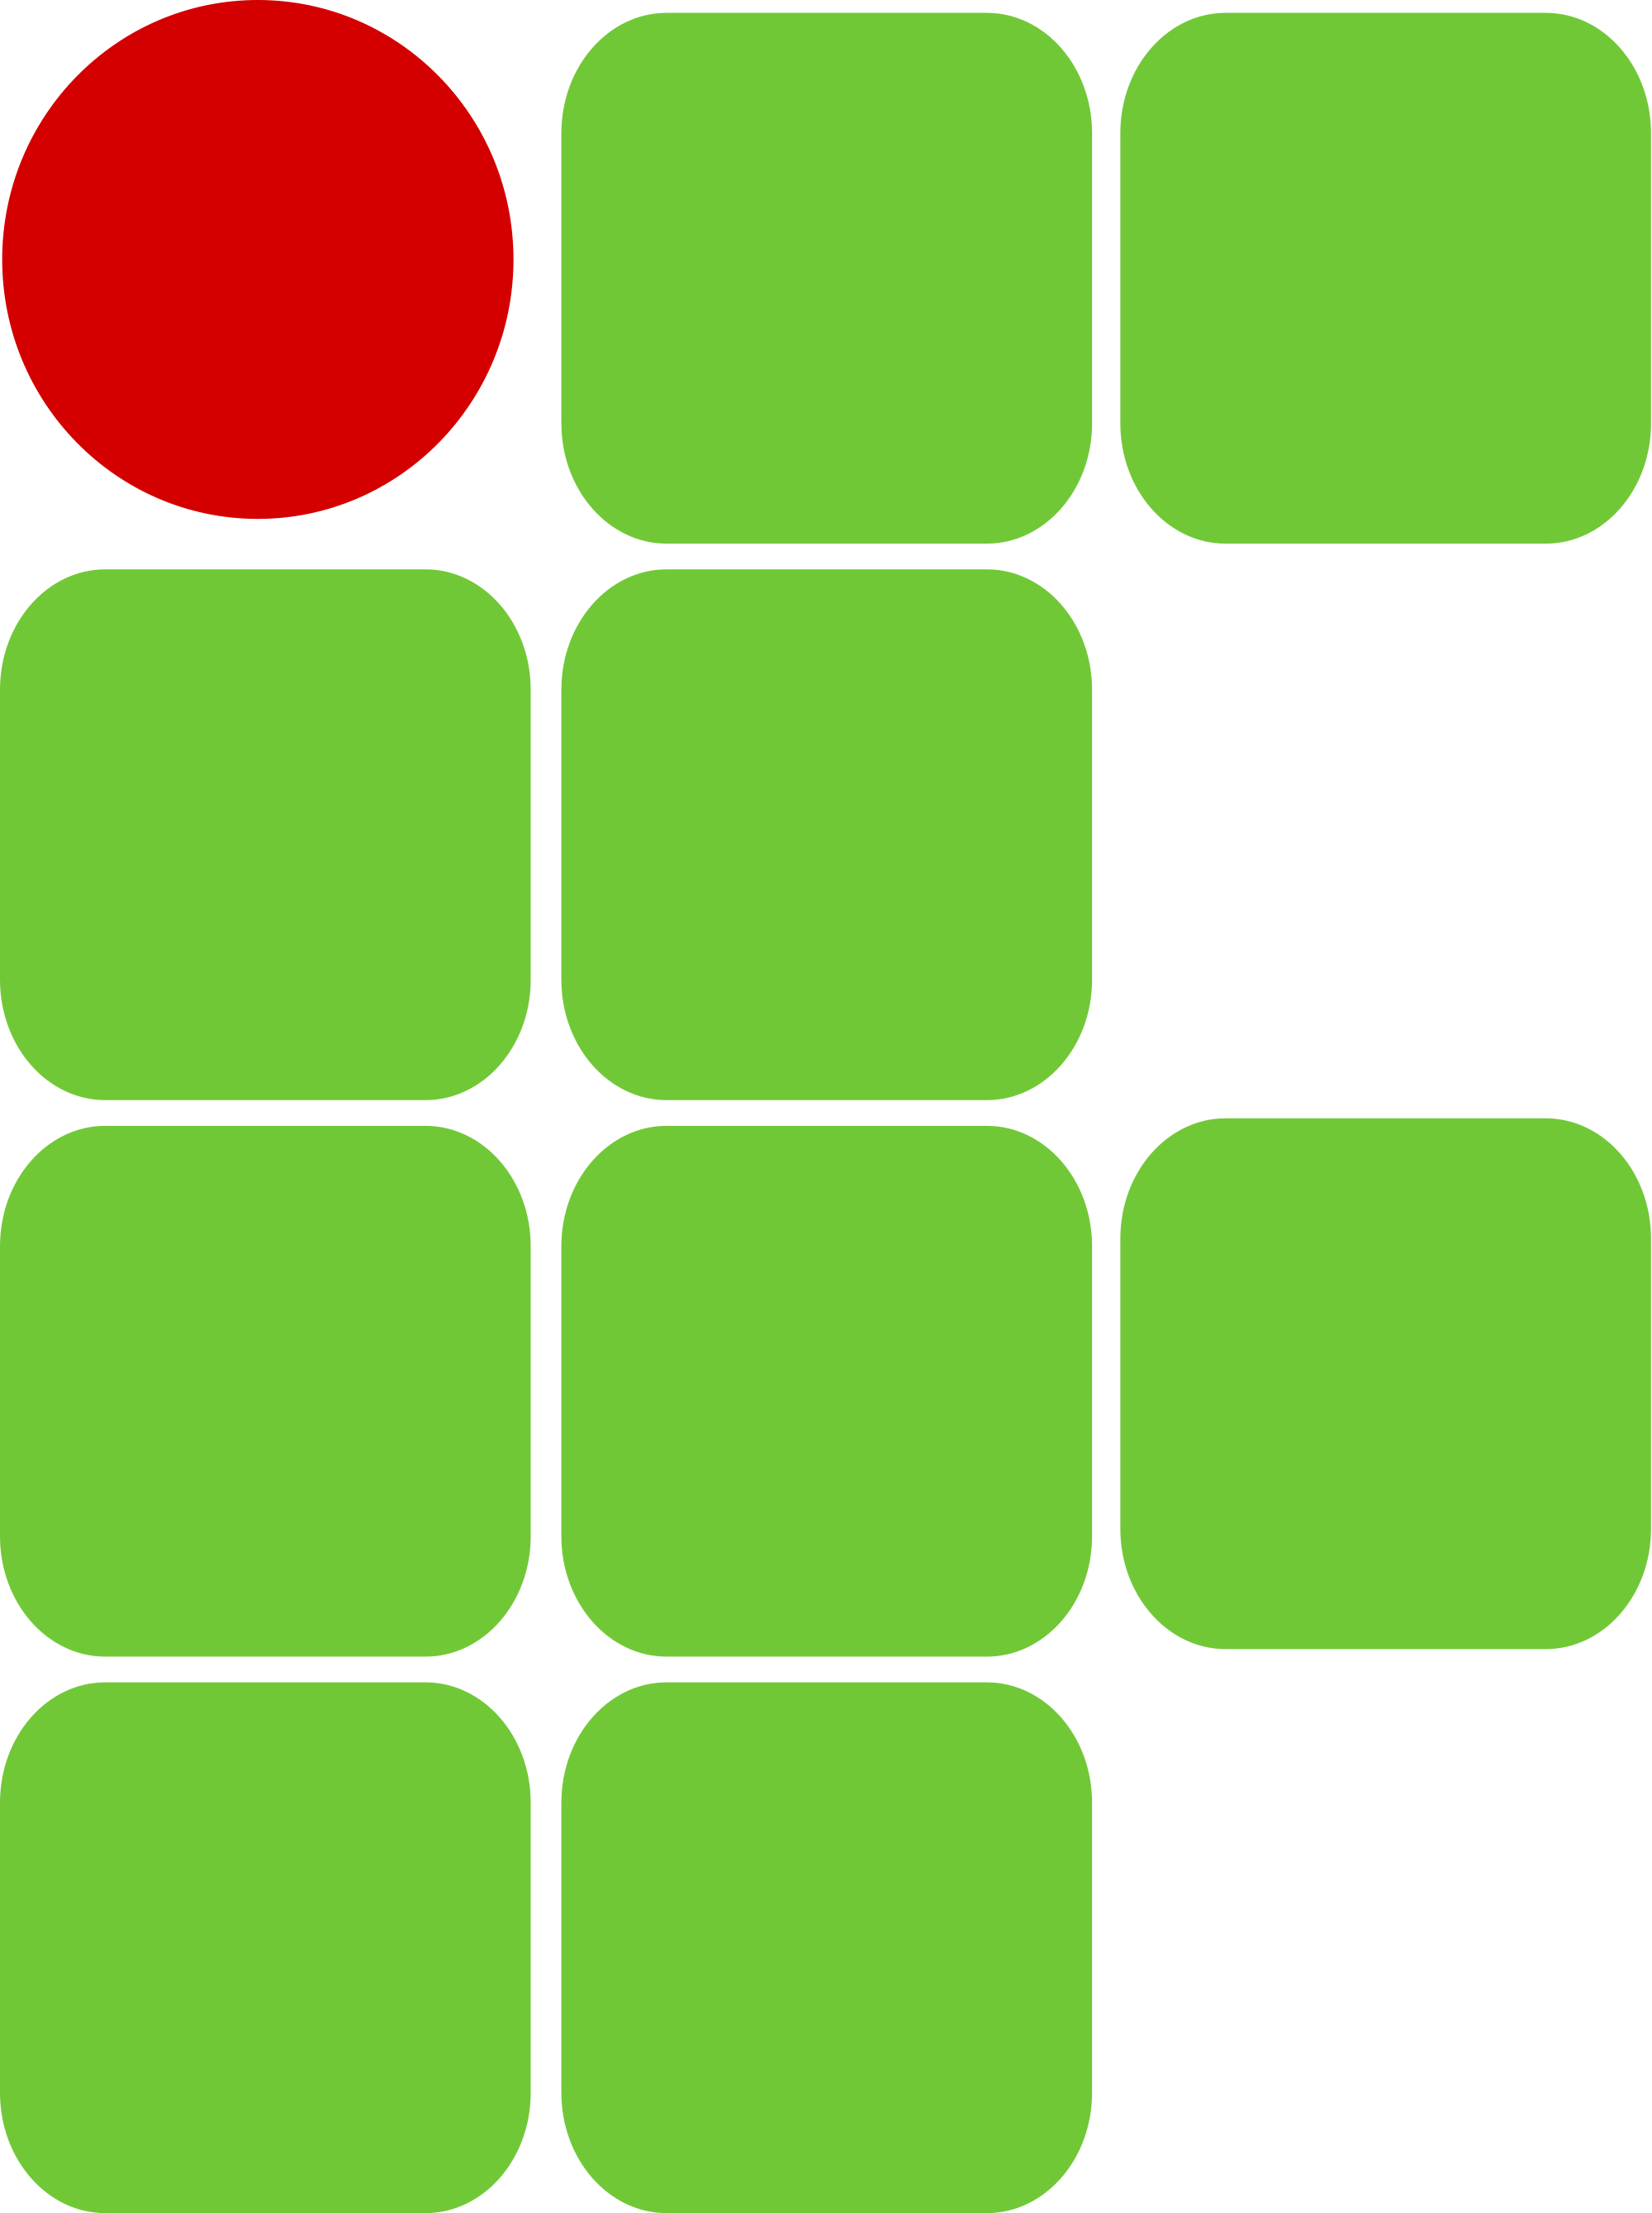
\includegraphics[height=0.7cm]{figs/logo.png}
% \end{textblock*}
% }

\setcounter{framenumber}{0}


% ----------------------------------------- %

\section{Plan}

\begin{frame}{Plan}

  \begin{itemize}[<+->]
    \item Overview of compilation of Java.
    \item Demo of compilation.
    \item Do some lab questions / Cover any material ye need help with.
  \end{itemize}

\end{frame}

\section{Compilation}
\subsection{What is compilation?}
\begin{frame}{Compilation in Java}

  Compiling code is the process of taking our programmer-readable 'source-code' and converting it to 'executable code'.

  \begin{exampleblock}{Examples}
    Linked lists, arrays e.t.c.
  \end{exampleblock}
\end{frame}

\subsection{Fun C Example}
\begin{frame}{``Hello world'' program in C}
  \inputminted{C}{code/main.c}
\end{frame}

\begin{frame}{Compiled ``Hello World'' Program from C to x86-64 machine code}
  \inputminted{objdump}{code/hello_world_hex}
\end{frame}

% \begin{frame}{Why use Data Structures?}
%   \begin{block}{Reason \#1}
%   Storing, managing and manipulating complex sets of data can be a burden on the programmer. A higher level abstraction like a data structure can help keep things simple when working at a higher level.
%   \end{block}
%   \begin{exampleblock}{Example}
%     Manipulating an image through a set of functions instead of through a multi-dimensional array.
%   \end{exampleblock}
% \end{frame}

% \begin{frame}{Why use Data Structures?}
% \begin{block}{Reason \#2}
%   There are many common patterns and activities in software. Algorithms and data structures are general utilities that can be used to solve a lot of common problems.
%   \end{block}
% \begin{exampleblock}{Example}
%   Sorting algorithm + Searching algorithm to get better speeds when searching for an item in a list.
% \end{exampleblock}
% \end{frame}

% \section{Big O}

% \begin{frame}{Big O Notation}
%   Big O notation is used to categorize algorithms by their performance when given a very large input. For example, in order to sort an array of 100 elements:
%   \medskip

% 	\begin{itemize}[<+->]
%     \item Bubble sort, with $O(n^2)$ will take $100^2 \Rightarrow 10,000$ units of time.
%     \item Quick sort, with $O(n \cdot \log 100)$ will take $n \cdot \log(100) \Rightarrow 200$ units of time.
%   \end{itemize}
%   \medskip
  
%   Big O notation signifies that the algorithm will never take longer than O (<whatever>) length of time.
% \end{frame}

% \begin{frame}{Common Big O functions}

% \begin{figure}
% \centering
% 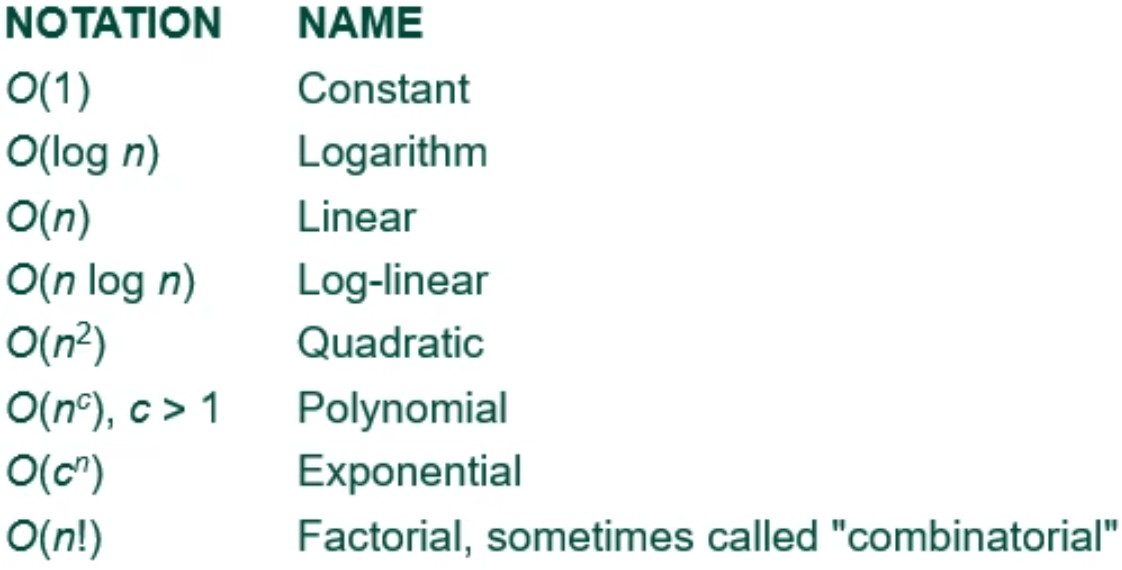
\includegraphics[width=0.8\linewidth]{figs/common_functions.png}

% \end{figure}

% \end{frame}

% \begin{frame}{Array List Functions}

% \begin{figure}
% \centering
% 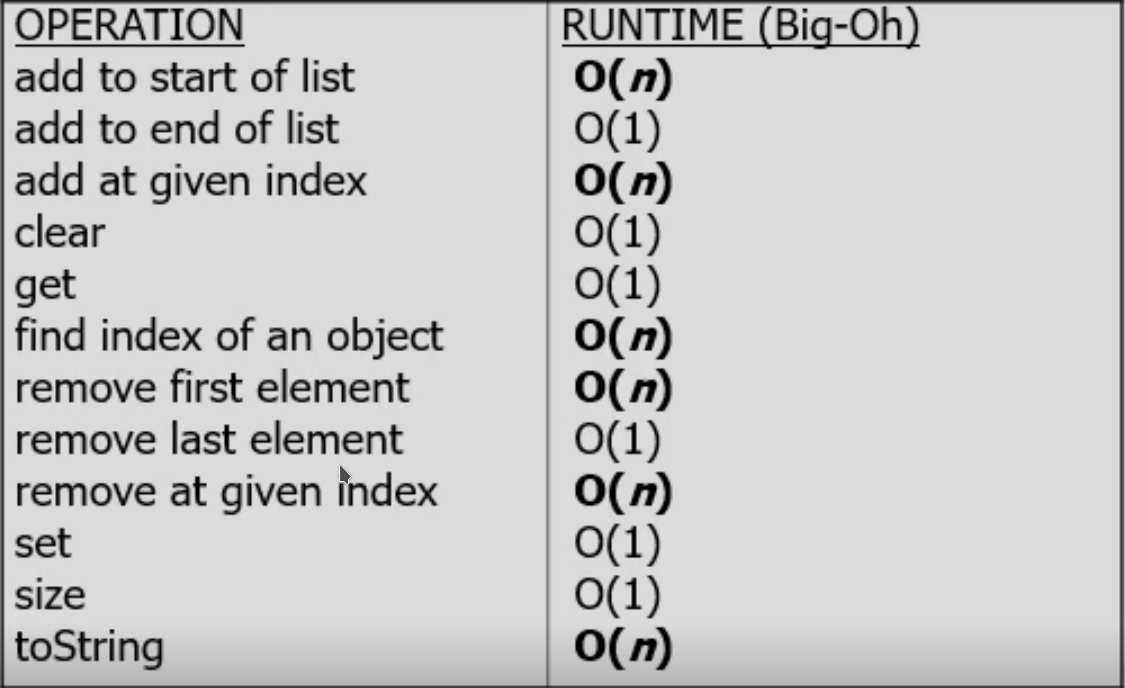
\includegraphics[width=0.8\linewidth]{figs/arraylist.png}

% \end{figure}

% \end{frame}

% \section{Command Line Arguments}

% \begin{frame}{Command Line Arguments}

% 	\begin{enumerate}[<+->]
%     \item Users can pass the arguments during the execution by passing the command-line arguments inside the main () method.
%     \item The arguments passed from the console can be received in the java program and it can be used as an input.
%     \item You can pass in any parameters such as String, double, int etc.
%     \item The arguments are converted into String and passed into the String args[] array declared in the main function.
%   \end{enumerate}
  
% \end{frame}

% \begin{frame}{Sample Programs}
%     \begin{block}{Sample Program \#1}
%         \inputminted{java}{code/prog1.java}
%     \end{block}
% \end{frame}

% \begin{frame}{Sample Program}
%   \begin{block}{Sample Program \#2}
%       \inputminted{java}{code/prog2.java}
%   \end{block}
% \end{frame}

\end{document}
